%Matteo Kumar - Leonard Schatt
% Fortgeschrittenes Physikalisches Praktikum

% Teilauswertung X

\section{$\alpha$-Spektroskopie}

\subsection{Energiekalibrierung}

Zunächst wurde das Spektrum von Radium-226 mit einer 1mm-Blende in einem Abstand von ca 5mm gemessen, um eine Relation zwischen Kanalnummer 
und Energieinhalt in diesem herzustellen. Dabei wurden die Daten des Files Kali\_ra226\_b1\_603 zunächst geplottet (Abb. \ref{bild:kali}) 
und mit den Werten aus der Tabelle in Abb. \ref{bild:TabelleRa} verglichen.

\begin{figure}[h]
    \centering
    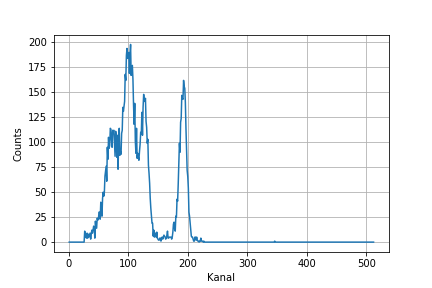
\includegraphics[scale=0.5]{Bilder/kali.png}
    \caption{Plot der Kalibrationsmessung} %Plot einfügen!!
    \label{bild:kali}
\end{figure}

\begin{figure}[h]
    \centering
    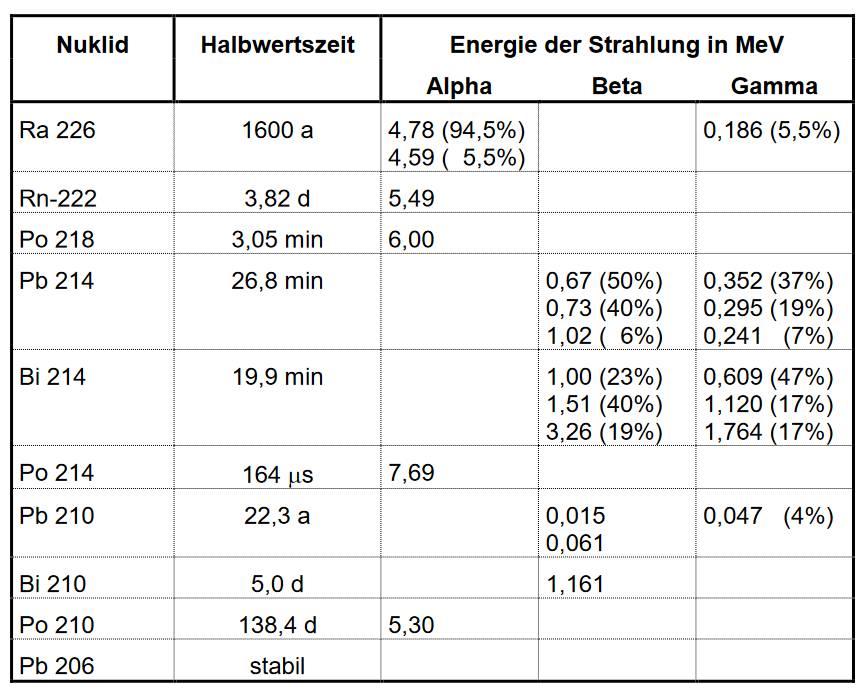
\includegraphics[scale=0.5]{Bilder/TabelleRadium.png}
    \caption{Zerfallsdaten der Ra-226-Reihe \protect \footnotemark}
    \label{bild:TabelleRa}
\end{figure}

\footnotetext{\cite{Kador2021}}

Dabei sind in der Tabelle zwei sehr kurzlebige Alphastrahler zu finden: Po-214 und Po-218. Da Po-214 die höchste Strahlenenergie hat, 
sollte der rechte einzelne Peak diesem Strahler zuzuordnen sein. Po-218 ist der rechte Peak des Dreifachpeaks zuzuordnen. Dessen 
linker Peak (Ra-226) ist für eine Kalibrierung zu schlecht aufgelöst und der mittlere aufgrund der Überlagerung zweier Strahler 
(Rn-222, Po-210) ebenfalls nicht geeignet
(\url{https://www.ld-didactic.de/software/524221en/Content/Appendix/Ra226.htm}, Stand: 14.09.21).

In den Daten wird nun der Kanal mit den maximalen Einträgen für jeden Peak gesucht. Dieser lag für Po-214 bei Kanal $193$ und 
für Po-218 bei Kanal $126$. Mit den Energie aus der Tabelle für Po-214 ($7,69$ MeV) und Po-218 ($6,00$ MeV) erhält man folgendes 
Gleichungssystem:

\begin{align*}{}
    7,69 MeV &= 193 \cdot m + E_0
    6,00 MeV &= 126 \cdot m + E_0
\end{align*}

Mit der Lösung:

\begin{equation*}
    m = 0,02522388 MeV, \qquad E_0 = 2,82179104 MeV
\end{equation*}

Womit sich die Kalibrierungsgerade ergibt zu:

\begin{equation}
    E = Kanalnummer \cdot 0,02522388 MeV + 2,82179104 MeV
\end{equation}


\subsection{Blendenverkleinerung}

\subsection{Absorption von $\alpha$-Strahlen}
